\chapter{Entwurfsmuster}

\section{Entwurfsmuster: Kompositum Pattern}

\textbf{Einsatz:} Die Memory-Hierarchie \code{Bit -> Nibble -> Byte -> Register} implementiert ein Composite Pattern, bei dem komplexere Speichereinheiten aus einfacheren zusammengesetzt werden.

\textbf{Beschreibung:}

\begin{itemize}
    \item \code{Bit} -- speichert einen einzelnen boolschen Wert
    \item \code{Nibble} -- besteht aus einem Array von 4 \code{Bit}-Objekten
    \item \code{Byte} -- besteht aus 2 \code{Nibble}-Objekten (High + Low)
    \item \code{Register} -- besteht aus 1 \code{Byte}-Objekt
\end{itemize}

Jede Ebene bietet Zugriffsmethoden auf ihrer Abstraktionsebene (\code{getBit()}, \code{getNibble()}, \code{getByte()}) und delegiert bei Bedarf an die darunterliegende Schicht. Ein \code{Byte} kann sowohl als Ganzes (\code{setByte(0xAB)}) als auch auf Nibble- oder Bitebene manipuliert werden.

\textbf{Begründung:} Die PIC-Hardware operiert auf verschiedenen Granularitätsebenen -- Einzelbits (Status-Flags), Nibbles (BCD-Operationen), Bytes (Registerwerte). Das Composite Pattern erlaubt einheitlichen Zugriff auf allen Ebenen, ohne die Implementierungsdetails zu verletzen.


\begin{center}
    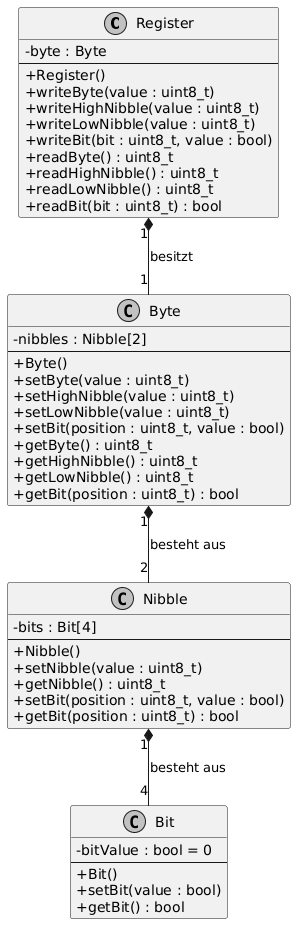
\includegraphics[width=0.5\textwidth]{UML/18.png}
\end{center}

\section{Entwurfsmuster: Strategy Pattern}

\textbf{Einsatz:} Die \code{Instruction}-Hierarchie implementiert das Strategy Pattern (bzw. Template Method Pattern) für die Ausführung verschiedener PIC-Instruktionen.

\textbf{Beschreibung:}

Die abstrakte Basisklasse \code{Instruction} definiert die Methode \code{virtual uint16_t execute() = 0}. Jede konkrete Instruktion (ADDWF, SUBWF, GOTO, CALL, BCF, BSF, etc.) implementiert ihren eigenen Algorithmus in \code{execute()}. Die \code{ALU} nutzt die Basisklasse als Schnittstelle und kann jede Instruktion polymorph ausführen, ohne den konkreten Typ zu kennen.

\begin{lstlisting}[style=codeblock,language=picassocpp]
// Strategy-Interface:
class Instruction {
    virtual uint16_t execute() = 0;
};

// Konkrete Strategien:
class ADDWF : public Arithmetic { uint16_t execute() override { /* Addition */ } };
class GOTO  : public Jump       { uint16_t execute() override { /* Sprung */ } };
class BCF   : public Bitwise    { uint16_t execute() override { /* Bit Clear */ } };

// Context (ALU):
class ALU {
    uint16_t executeInstruction(Instruction& instr) {
        return instr.execute();  // polymorphe Ausführung
    }
};
\end{lstlisting}

\textbf{Begründung:} Der PIC hat 35+ unterschiedliche Instruktionen, die alle denselben Lebenszyklus durchlaufen (Dekodierung $\rightarrow$ Ausführung $\rightarrow$ Zyklenanzahl), aber völlig unterschiedliche Algorithmen haben. Das Strategy Pattern ermöglicht das Hinzufügen neuer Instruktionen durch Erstellung neuer Klassen, ohne bestehenden Code zu ändern.


\begin{center}
    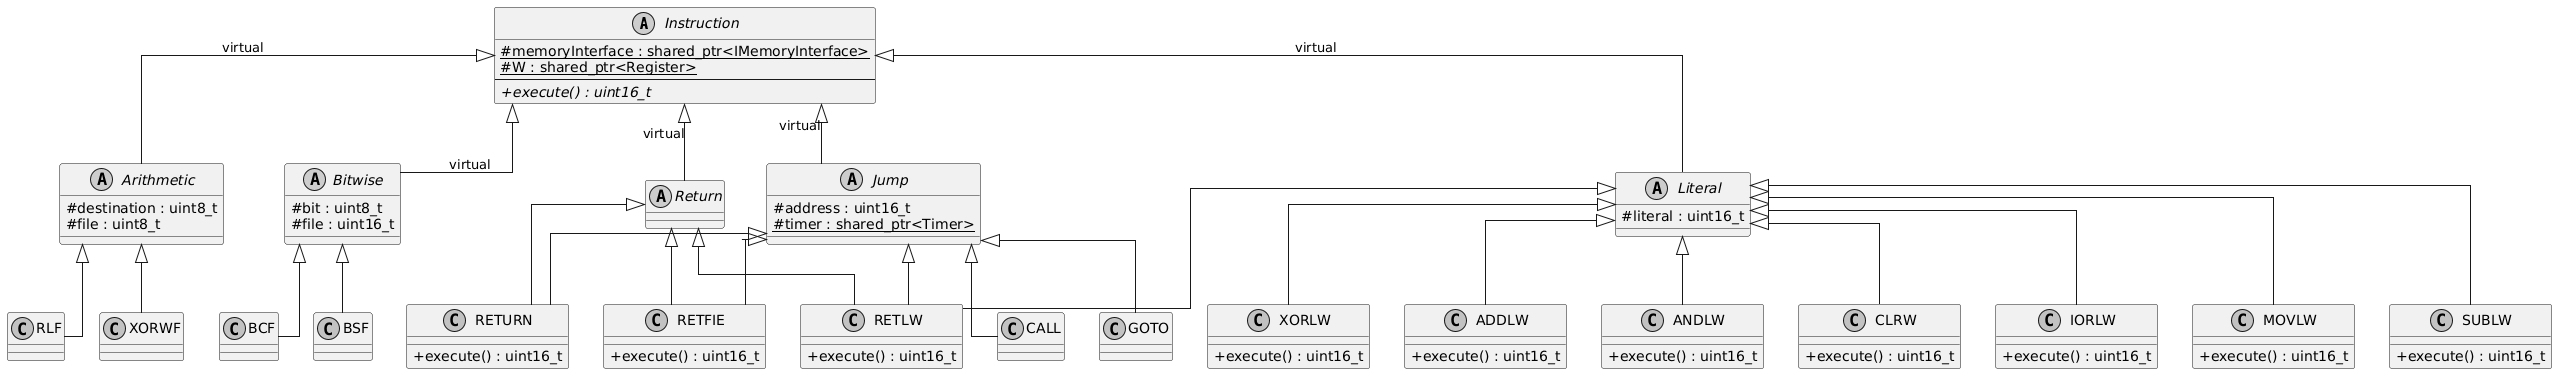
\includegraphics[height=0.25\textwidth, angle=90]{UML/19.png}
\end{center}

